\documentclass{article}

\usepackage{amsmath,amssymb,mathtools,multirow,graphicx}
\usepackage[ruled,vlined,linesnumbered]{algorithm2e}
\usepackage{algorithmic}
\usepackage{float}


\title{\bf Shi(f)t happens}
\author{Manuel Baumann}
\date{September 1, 2015}
\begin{document}
 \maketitle
 My PhD research mostly focuses on the efficient numerical solution of so-called \textit{shifted linear systems} which are of the form,
 \begin{align}
 \label{shifted}
  (A - \omega_k I) \mathbf{x}_k = \mathbf{b}, \quad \text{where } k = 1,...,n_\omega,
 \end{align}
 and where $A$ is an $n \times n$ matrix, and $I$ is the identity of the same size. As we see from \eqref{shifted}, we are looking for $n_\omega$ solutions $\mathbf{x}_1,..., \mathbf{x}_{n_\omega}$ where the system matrix only differs by a constant shift on the diagonal. Typically, $n_\omega$ is of the order of ten, while in a large-scale simulation $n$ can be several millions. Shifted systems are an interesting subject! For example, they have the same eigenspace with spectrum that is shifted by $\omega_k$. Can you show this?
 \section{Application}
 Shifted linear systems arise in seismic exploration.
 \begin{figure}[ht]
  \centering
  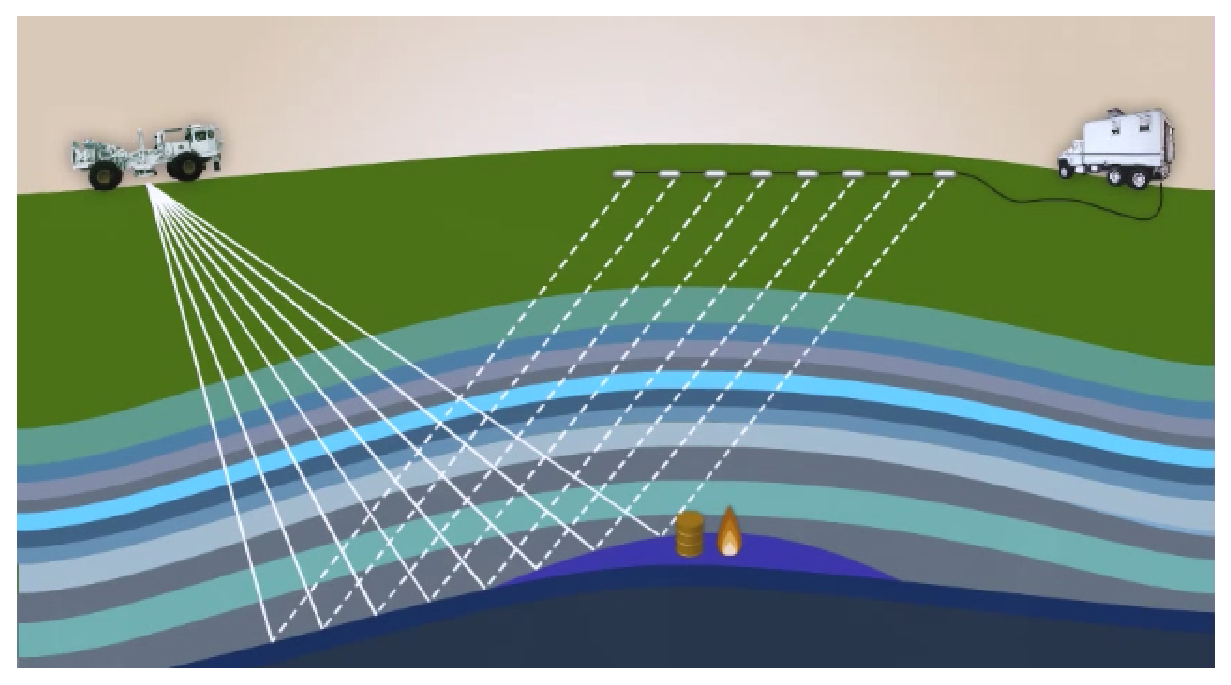
\includegraphics[width=0.5\textwidth]{figs/Seismic}
  \caption{Sender and receiver \copyright ScienceRocks!} \label{Seimics}
 \end{figure}
 \section{GMRES for shifted systems}
 Krylov subspace,
 \begin{align*}
  \mathcal{K}_m(A,\mathbf{b}) := \text{span} \{\mathbf{b}, A \mathbf{b}, A^2 \mathbf{b},...,A^{m-1}\mathbf{b} \}
 \end{align*}
 Arnoldi algorithm,

\begin{algorithm}[H]
\caption{The Arnoldi algorithm, \cite{GL96}}
\label{alg:Arn}
\begin{algorithmic}
\FOR{$j = 1$ to $m$}
\STATE Compute $\mathbf{w} = A \mathbf{v}_j$
\FOR{$i = 1$ to $j$}
\STATE $h_{i,j} = \mathbf{w}^{\mathsf{T}} \mathbf{v}_i$
\STATE $\mathbf{w} = \mathbf{w} - h_{i,j} \mathbf{v}_i$
\ENDFOR
\ENDFOR
\end{algorithmic}
\end{algorithm}

 \begin{align*}
 AV_m = V_{m+1}\underbar{H}_m
 \end{align*}
 Minimize residual,
 \begin{align*}
 \mathbf{x}_m &= \min_{\mathbf{x} \in \mathcal{K}_m} \| \mathbf{b} - A \mathbf{x}\|
              = \min_{\mathbf{y} \in \mathbb{R}^m} \| \mathbf{b} - A V_m\mathbf{y}\| \\
              &= \min_{x \in \mathcal{K}_m} \| \mathbf{b} - A \mathbf{x}\|
 \end{align*}
 \cite{GL96}
 
 Shifted version \cite{F98} solve the same with shifted Hessenberg matrix $\underbar{H}_m^{(\omega_k)} = \underbar{H}_m - \omega_k \underbar{I}$. This has the advantage 
 \section{Nested Krylov methods}
 \cite{BG14}
 \bibliographystyle{siam}
 \bibliography{LitColl.bib}

\end{document}
